\section{Threat Model}
    The microarchitectural techniques for timing channel protection discussed 
    in this work are broad and can be applied to a wide range of applications.  
    This section describes the general security goals that this architecture 
    supports for all domains, although the threat model may vary depending on 
    the specific application. For each application, this architecture aims to 
    thwart adversaries that can carry out software attacks including attacks
    that exploit timing channels. This is achieved by applying the 
    microarchitectural timing channel countermeasures proposed in this work in 
    conjunction with existing techniques to control explicit information flows. 
    This work is not concerned with attacks that require physical access to the 
    device such as differential power analysis. Physical attacks are inherently 
    limited to domains where it is likely that the adversary can physically 
    posess the device, and preventing all attacks of this kind is too costly 
    for many applications.

    We present a new primitive to isolate software modules that might otherwise 
    leak information through timing channels called a timing compartment.  A 
    timing compartment consists of one or more software modules (such as 
    processes or threads in a single OS system or virtual machines in a 
    virtualization based system).  Software modules within the same timing 
    compartment may leak information through timing channels (e.g. because they 
    trust eachother), but timing channels between timing compartments must be 
    controlled according to a policy that meets the security requirements of 
    the system. This policy entails of a lattice of security levels such as 
    $\mathtt{normal} \sqsubseteq \mathtt{secure}$, where the information 
    available to a timing compartment includes any information available to 
    timing compartments with an equal security level and with levels that 
    preceed it in the lattice order. 

    Timing compartments do not necessarily have to control explicit information 
    flows, but rather separate primitives may be used to control these. For 
    example, a system may similarly group software modules into explicit flow 
    compartments that are similar to timing compartments, but control 
    communication through explicit information flows. Although it is often 
    desirable for the timing compartments of a system to completely coincide 
    witht he explicit flow compartments, there are advantages to providing 
    separate, isolating primtives. When designing a secure system, implementors 
    must consider how the cost required to carry out a particular attack 
    compares with other attacks, the potential damage that could be caused by 
    an attack, and the cost and performance impact of implementing the security 
    mechanisms needed to stop it. Separating the primitives that control timing 
    channels and explicit information flows allows system implementors the 
    flexibility to omit certain timing channel attacks from the threat model 
    while handling other attacks separately.

\subsection{Baseline Architecture}

    \begin{figure}
        \begin{center}
            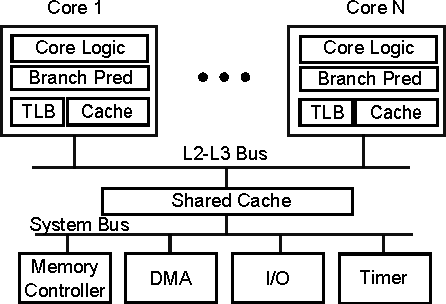
\includegraphics[width=3in]{figs/baseline.pdf}
            \caption{The timing-channel vulnerable baseline architecture.}
            \label{fig:baseline}
        \end{center}
    \end{figure}

    Figure \ref{fig:baseline} shows the baseline architecture which is later 
    extended to include timing channel protection. The architecture has 
    multiple cores, each with a branch predictor, one or more private caches, a 
    TLB, and the core logic. Each processor is connected to a shared cache 
    through an on-chip network. The multicore processor is connected to the 
    main memory and a DMA module through the system bus. 

    The hardware is concurrently shared by multiple timing compartments. As 
    shown in Figure \ref{fig:baseline}, it is possible for a timing compartment 
    to have multiple software modules which may be allocated to different 
    cores. It is also possible for timing compartments to be time multiplexd on 
    the same core (e.g.  by context switching VMs), but it is not possible for 
    timing compartments to execute concurrently on the same core (e.g. through 
    SMT).

